\documentclass{standalone}
\usepackage{tikz}

% == Tikz
\newcommand{\drawcirc}{\node[draw,circle,minimum size=1.5cm]}
\newcommand{\drawbox}{\node[draw,rectangle,minimum size=1.5cm]}
\newcommand{\drawdummy}{\node[minimum size=0,inner sep=0]}
\newcommand{\zeroSink}{\mathsf{o}}
\newcommand{\target}{\mathsf{f}}

\begin{document}
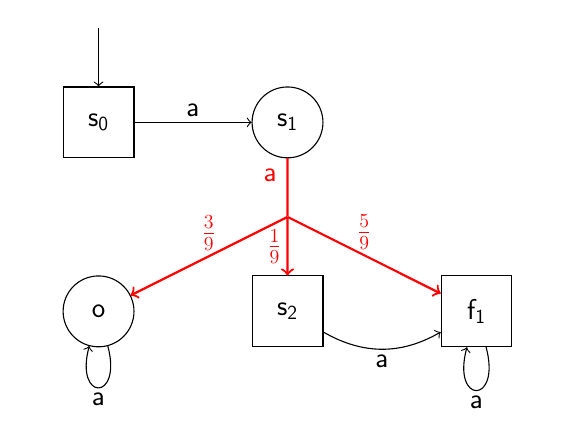
\begin{tikzpicture}[scale=0.6, every node/.style={font=\LARGE, transform shape}]
%little BCEC with loop
\drawdummy (init) at (0,2) {};
\drawdummy (spacing1) at (9.5,-2) {};
\drawdummy (space3) at (0,1.5) {};
\drawdummy (spacing2) at (-1.5,-2) {};
\drawbox (q) at (0,0) {$\mathsf{s_0}$};
\drawcirc (p) at (4,0) {$\mathsf{s_1}$};
\drawdummy (mid) at (4,-2) {};
\drawbox (11) at (8,-4) {$\mathsf{f_1}$};
\drawbox (12) at (4,-4) {$\mathsf{s_2}$};
\drawcirc (0) at (0,-4)  {$\mathrm{\zeroSink}$};

\draw[->] (init) to (q);
\draw[->]  (q) to node [above ,midway] {$\mathsf{a}$}(p);

\draw[thick, red, -] (p) to node [text width =1.0cm, above, midway] {$\mathsf{a}$}(mid);

\draw[thick, red, ->] (mid) to node [midway, above] {$\frac{3}{9}$} (0);
\draw[thick, red, ->] (mid) to node [midway, above] {$\frac{5}{9}$} (11);
\draw[thick, red, ->] (mid) to node [midway, left] {$\frac{1}{9}$} (12);

\draw[->]  (0) to[loop below]  node [midway,below] {$\mathsf{a}$} (0);
\draw[->]  (11) to [loop below] node [midway,below] {$\mathsf{a}$} (11);
\draw[->] (12) to [bend right] node [midway,below] {$\mathsf{a}$} (11);
\end{tikzpicture}
\end{document}
